\documentclass{beamer}\usepackage[]{graphicx}\usepackage[]{color}
%% maxwidth is the original width if it is less than linewidth
%% otherwise use linewidth (to make sure the graphics do not exceed the margin)
\makeatletter
\def\maxwidth{ %
  \ifdim\Gin@nat@width>\linewidth
    \linewidth
  \else
    \Gin@nat@width
  \fi
}
\makeatother

\definecolor{fgcolor}{rgb}{0.345, 0.345, 0.345}
\newcommand{\hlnum}[1]{\textcolor[rgb]{0.686,0.059,0.569}{#1}}%
\newcommand{\hlstr}[1]{\textcolor[rgb]{0.192,0.494,0.8}{#1}}%
\newcommand{\hlcom}[1]{\textcolor[rgb]{0.678,0.584,0.686}{\textit{#1}}}%
\newcommand{\hlopt}[1]{\textcolor[rgb]{0,0,0}{#1}}%
\newcommand{\hlstd}[1]{\textcolor[rgb]{0.345,0.345,0.345}{#1}}%
\newcommand{\hlkwa}[1]{\textcolor[rgb]{0.161,0.373,0.58}{\textbf{#1}}}%
\newcommand{\hlkwb}[1]{\textcolor[rgb]{0.69,0.353,0.396}{#1}}%
\newcommand{\hlkwc}[1]{\textcolor[rgb]{0.333,0.667,0.333}{#1}}%
\newcommand{\hlkwd}[1]{\textcolor[rgb]{0.737,0.353,0.396}{\textbf{#1}}}%
\let\hlipl\hlkwb

\usepackage{framed}
\makeatletter
\newenvironment{kframe}{%
 \def\at@end@of@kframe{}%
 \ifinner\ifhmode%
  \def\at@end@of@kframe{\end{minipage}}%
  \begin{minipage}{\columnwidth}%
 \fi\fi%
 \def\FrameCommand##1{\hskip\@totalleftmargin \hskip-\fboxsep
 \colorbox{shadecolor}{##1}\hskip-\fboxsep
     % There is no \\@totalrightmargin, so:
     \hskip-\linewidth \hskip-\@totalleftmargin \hskip\columnwidth}%
 \MakeFramed {\advance\hsize-\width
   \@totalleftmargin\z@ \linewidth\hsize
   \@setminipage}}%
 {\par\unskip\endMakeFramed%
 \at@end@of@kframe}
\makeatother

\definecolor{shadecolor}{rgb}{.97, .97, .97}
\definecolor{messagecolor}{rgb}{0, 0, 0}
\definecolor{warningcolor}{rgb}{1, 0, 1}
\definecolor{errorcolor}{rgb}{1, 0, 0}
\newenvironment{knitrout}{}{} % an empty environment to be redefined in TeX

\usepackage{alltt}
\usecolortheme{albatross}
\IfFileExists{upquote.sty}{\usepackage{upquote}}{}
\begin{document}

\title{Comparison Barplots with The Shunned House}
\author{Andrew Innes}

\begin{frame}
  \titlepage
\end{frame}

\begin{frame}
  \frametitle{Outline}
    \tableofcontents
\end{frame}

\section{Install and Load Libraries}
\begin{frame}[fragile]
  \frametitle{Install and Load Libraries}
    \begin{itemize}
      \item<1->
\begin{knitrout}
\definecolor{shadecolor}{rgb}{0.969, 0.969, 0.969}\color{fgcolor}\begin{kframe}
\begin{alltt}
\hlkwd{library}\hlstd{(dplyr)}
\end{alltt}
\end{kframe}
\end{knitrout}
      \item<2->
\begin{knitrout}
\definecolor{shadecolor}{rgb}{0.969, 0.969, 0.969}\color{fgcolor}\begin{kframe}
\begin{alltt}
\hlkwd{library}\hlstd{(tidytext)}
\end{alltt}
\end{kframe}
\end{knitrout}
      \item<3->
\begin{knitrout}
\definecolor{shadecolor}{rgb}{0.969, 0.969, 0.969}\color{fgcolor}\begin{kframe}
\begin{alltt}
\hlkwd{library}\hlstd{(gutenbergr)}
\end{alltt}
\end{kframe}
\end{knitrout}
      \item<4->
\begin{knitrout}
\definecolor{shadecolor}{rgb}{0.969, 0.969, 0.969}\color{fgcolor}\begin{kframe}
\begin{alltt}
\hlkwd{library}\hlstd{(ggplot2)}
\end{alltt}
\end{kframe}
\end{knitrout}
      \item<5->
\begin{knitrout}
\definecolor{shadecolor}{rgb}{0.969, 0.969, 0.969}\color{fgcolor}\begin{kframe}
\begin{alltt}
\hlkwd{library}\hlstd{(stringr)}
\end{alltt}
\end{kframe}
\end{knitrout}
    \end{itemize}
\end{frame}
      
\section{Access Project Gutenberg}
\begin{frame}[fragile]
  \frametitle{Access Project Gutenberg}
\begin{knitrout}
\definecolor{shadecolor}{rgb}{0.969, 0.969, 0.969}\color{fgcolor}\begin{kframe}
\begin{alltt}
\hlstd{df}\hlkwb{<-}\hlkwd{gutenberg_works}\hlstd{(}\hlkwd{str_detect}\hlstd{(title,}
                               \hlstr{'The Shunned House'}\hlstd{))}
\hlstd{df}\hlopt{$}\hlstd{gutenberg_id}
\end{alltt}
\begin{verbatim}
## [1] 31469
\end{verbatim}
\begin{alltt}
\hlstd{df}\hlopt{$}\hlstd{title}
\end{alltt}
\begin{verbatim}
## [1] "The Shunned House"
\end{verbatim}
\end{kframe}
\end{knitrout}
\end{frame}

\section{Download The Shunned House}
\begin{frame}[fragile]
  \frametitle{Download The Shunned House}
\begin{knitrout}
\definecolor{shadecolor}{rgb}{0.969, 0.969, 0.969}\color{fgcolor}\begin{kframe}
\begin{alltt}
\hlstd{House}\hlkwb{<-}\hlkwd{gutenberg_download}\hlstd{(}\hlnum{31469}\hlstd{)}
\hlkwd{colnames}\hlstd{(House)}
\end{alltt}
\begin{verbatim}
## [1] "gutenberg_id" "text"
\end{verbatim}
\begin{alltt}
\hlkwd{substr}\hlstd{(House}\hlopt{$}\hlstd{text[}\hlnum{400}\hlstd{],}\hlnum{1}\hlstd{,}\hlnum{21}\hlstd{)}
\end{alltt}
\begin{verbatim}
## [1] "of mold in that regio"
\end{verbatim}
\end{kframe}
\end{knitrout}
\end{frame}

\section{Unpack the Words}
\begin{frame}[fragile]
  \frametitle{Unpack the Words}
\begin{knitrout}
\definecolor{shadecolor}{rgb}{0.969, 0.969, 0.969}\color{fgcolor}\begin{kframe}
\begin{alltt}
\hlstd{shunned_words}\hlkwb{<-}\hlstd{House}\hlopt
  \hlkwd{unnest_tokens}\hlstd{(word,text)}
\hlkwd{colnames}\hlstd{(shunned_words)}
\end{alltt}
\begin{verbatim}
## [1] "gutenberg_id" "word"
\end{verbatim}
\begin{alltt}
\hlstd{shunned_words[}\hlnum{398}\hlopt{:}\hlnum{400}\hlstd{,]}
\end{alltt}
\begin{verbatim}
## # A tibble: 3 x 2
##   gutenberg_id  word
##          <int> <chr>
## 1        31469  farm
## 2        31469    or
## 3        31469  semi
\end{verbatim}
\end{kframe}
\end{knitrout}
\end{frame}

\section{The Bing Lexicon}
\begin{frame}[fragile]
  \frametitle{The Bing Lexicon}
\begin{knitrout}
\definecolor{shadecolor}{rgb}{0.969, 0.969, 0.969}\color{fgcolor}\begin{kframe}
\begin{alltt}
\hlstd{bing}\hlkwb{<-}\hlkwd{get_sentiments}\hlstd{(}\hlstr{'bing'}\hlstd{)}
\hlkwd{colnames}\hlstd{(bing)}
\end{alltt}
\begin{verbatim}
## [1] "word"      "sentiment"
\end{verbatim}
\begin{alltt}
\hlstd{bing[}\hlnum{398}\hlopt{:}\hlnum{400}\hlstd{,]}
\end{alltt}
\begin{verbatim}
## # A tibble: 3 x 2
##          word sentiment
##         <chr>     <chr>
## 1     awkward  negative
## 2 awkwardness  negative
## 3      awsome  positive
\end{verbatim}
\end{kframe}
\end{knitrout}
\end{frame}

\section{The Inner Join}
\begin{frame}[fragile]
  \frametitle{The Inner Join}
\begin{knitrout}
\definecolor{shadecolor}{rgb}{0.969, 0.969, 0.969}\color{fgcolor}\begin{kframe}
\begin{alltt}
\hlstd{shunned_words}\hlkwb{<-}\hlkwd{inner_join}\hlstd{(shunned_words,bing)}
\hlstd{shunned_words}\hlopt{$}\hlstd{gutenberg_id}\hlkwb{<-}\hlkwa{NULL}
\hlstd{shunned_words[}\hlnum{398}\hlopt{:}\hlnum{400}\hlstd{,]}
\end{alltt}
\begin{verbatim}
## # A tibble: 3 x 2
##       word sentiment
##      <chr>     <chr>
## 1 ignorant  negative
## 2 smelling  negative
## 3  shunned  negative
\end{verbatim}
\end{kframe}
\end{knitrout}
\end{frame}

\section{Top Ten Positive Words}
\begin{frame}[allowframebreaks,fragile]
  \frametitle{Top Ten Positive Words}
\begin{knitrout}
\definecolor{shadecolor}{rgb}{0.969, 0.969, 0.969}\color{fgcolor}\begin{kframe}
\begin{alltt}
\hlstd{shunned_pos}\hlkwb{<-}\hlstd{shunned_words}\hlopt
  \hlkwd{filter}\hlstd{(sentiment}\hlopt{==}\hlstr{'positive'}\hlstd{)}\hlopt
  \hlkwd{group_by}\hlstd{(word)}\hlopt
  \hlkwd{summarize}\hlstd{(}\hlkwc{count}\hlstd{=}\hlkwd{n}\hlstd{(),}\hlkwc{sentiment}\hlstd{=}\hlkwd{first}\hlstd{(sentiment))}\hlopt
  \hlkwd{arrange}\hlstd{(count)}\hlopt
  \hlkwd{top_n}\hlstd{(}\hlnum{10}\hlstd{,}\hlkwc{wt}\hlstd{=count)}
\end{alltt}
\end{kframe}
\end{knitrout}
\framebreak
\begin{knitrout}
\definecolor{shadecolor}{rgb}{0.969, 0.969, 0.969}\color{fgcolor}\begin{kframe}
\begin{alltt}
\hlstd{shunned_pos}
\end{alltt}
\begin{verbatim}
## # A tibble: 13 x 3
##          word count sentiment
##         <chr> <int>     <chr>
##  1     enough     4  positive
##  2       good     4  positive
##  3        led     4  positive
##  4     master     4  positive
##  5     strong     4  positive
##  6  strongest     4  positive
##  7     proper     5  positive
##  8 providence     8  positive
##  9       well     9  positive
## 10      mercy    10  positive
## 11      great    12  positive
## 12    benefit    13  positive
## 13       like    17  positive
\end{verbatim}
\end{kframe}
\end{knitrout}
\end{frame}

\section{Top Ten Negative Words}
\begin{frame}[allowframebreaks,fragile]
  \frametitle{Top Ten Negative Words}
\begin{knitrout}
\definecolor{shadecolor}{rgb}{0.969, 0.969, 0.969}\color{fgcolor}\begin{kframe}
\begin{alltt}
\hlstd{shunned_neg}\hlkwb{<-}\hlstd{shunned_words}\hlopt
  \hlkwd{filter}\hlstd{(sentiment}\hlopt{==}\hlstr{'negative'}\hlstd{)}\hlopt
  \hlkwd{group_by}\hlstd{(word)}\hlopt
  \hlkwd{summarize}\hlstd{(}\hlkwc{count}\hlstd{=}\hlkwd{n}\hlstd{(),}\hlkwc{sentiment}\hlstd{=}\hlkwd{first}\hlstd{(sentiment))}\hlopt
  \hlkwd{arrange}\hlstd{(count)}\hlopt
  \hlkwd{filter}\hlstd{(word}\hlopt{!=}\hlstr{'miss'}\hlstd{)}\hlopt
  \hlkwd{top_n}\hlstd{(}\hlnum{10}\hlstd{,}\hlkwc{wt}\hlstd{=count)}
\end{alltt}
\end{kframe}
\end{knitrout}
\framebreak
\begin{knitrout}
\definecolor{shadecolor}{rgb}{0.969, 0.969, 0.969}\color{fgcolor}\begin{kframe}
\begin{alltt}
\hlstd{shunned_neg}
\end{alltt}
\begin{verbatim}
## # A tibble: 14 x 3
##        word count sentiment
##       <chr> <int>     <chr>
##  1   broken     5  negative
##  2     evil     5  negative
##  3 horrible     5  negative
##  4 peculiar     5  negative
##  5 sinister     5  negative
##  6    smell     5  negative
##  7 terrible     5  negative
##  8    weird     5  negative
##  9  hideous     7  negative
## 10    queer     8  negative
## 11    death     9  negative
## 12  strange    10  negative
## 13     died    11  negative
## 14  shunned    19  negative
\end{verbatim}
\end{kframe}
\end{knitrout}
\end{frame}

\section{The Comparison Bar Plot}
\begin{frame}[allowframebreaks,fragile]
  \frametitle{The Comparison Bar Plot}
\begin{knitrout}
\definecolor{shadecolor}{rgb}{0.969, 0.969, 0.969}\color{fgcolor}\begin{kframe}
\begin{alltt}
\hlstd{shunned_pos}\hlopt{$}\hlstd{word}\hlkwb{<-}\hlkwd{factor}\hlstd{(shunned_pos}\hlopt{$}\hlstd{word,}
                         \hlkwc{levels}\hlstd{=shunned_pos}\hlopt{$}\hlstd{word)}
\hlstd{shunned_neg}\hlopt{$}\hlstd{word}\hlkwb{<-}\hlkwd{factor}\hlstd{(shunned_neg}\hlopt{$}\hlstd{word,}
                         \hlkwc{levels}\hlstd{=shunned_neg}\hlopt{$}\hlstd{word)}
\hlstd{shunned_comp}\hlkwb{<-}\hlkwd{rbind}\hlstd{(shunned_pos,shunned_neg)}
\hlstd{plot}\hlkwb{<-}\hlkwd{ggplot}\hlstd{()}\hlopt{+}
  \hlkwd{geom_bar}\hlstd{(}\hlkwc{data}\hlstd{=shunned_comp,}
           \hlkwd{aes}\hlstd{(}\hlkwc{x}\hlstd{=word,}\hlkwc{y}\hlstd{=count,} \hlkwc{fill}\hlstd{=sentiment,}
               \hlkwc{color}\hlstd{=sentiment),}\hlkwc{stat}\hlstd{=}\hlstr{'identity'}\hlstd{)}\hlopt{+}
  \hlkwd{coord_flip}\hlstd{()}\hlopt{+}
  \hlkwd{facet_wrap}\hlstd{(}\hlopt{~}\hlstd{sentiment,}\hlkwc{scales}\hlstd{=}\hlstr{'free_y'}\hlstd{)}\hlopt{+}
  \hlkwd{scale_fill_manual}\hlstd{(}\hlkwc{values}\hlstd{=}\hlkwd{c}\hlstd{(}\hlstr{'black'}\hlstd{,}\hlstr{'#ea6205'}\hlstd{))}\hlopt{+}
  \hlkwd{scale_color_manual}\hlstd{(}\hlkwc{values}\hlstd{=}\hlkwd{c}\hlstd{(}\hlstr{'#ea6205'}\hlstd{,}\hlstr{'black'}\hlstd{))}
\end{alltt}
\end{kframe}
\end{knitrout}
\framebreak
\begin{knitrout}
\definecolor{shadecolor}{rgb}{0.969, 0.969, 0.969}\color{fgcolor}
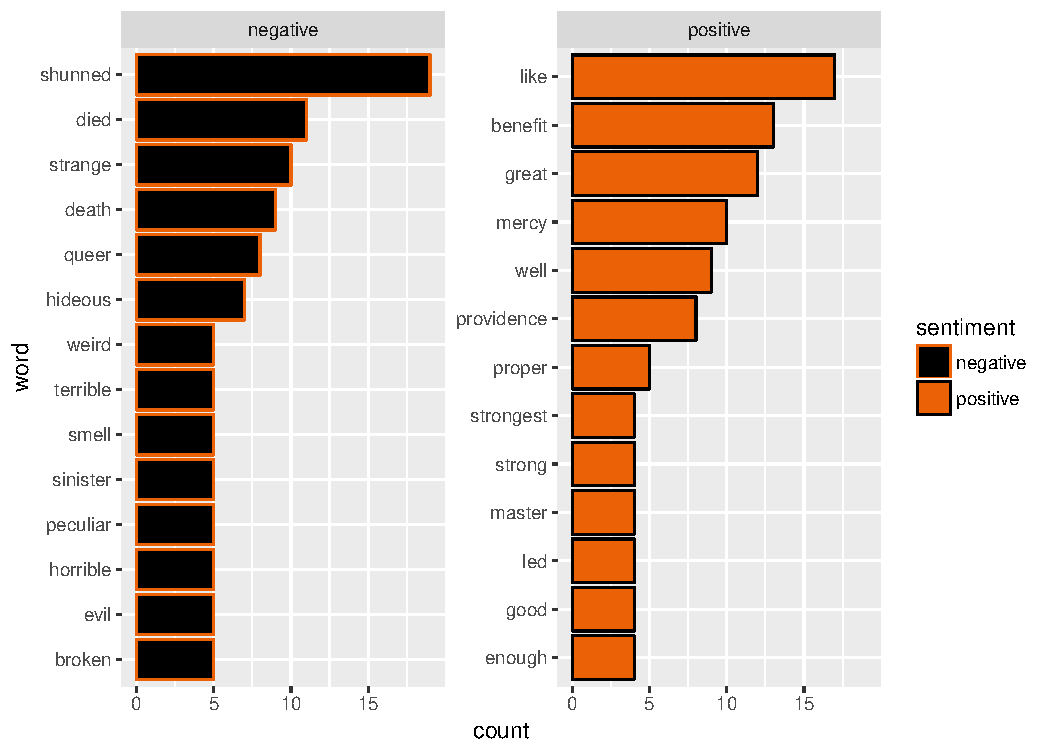
\includegraphics[width=\maxwidth]{figure/unnamed-chunk-16-1} 

\end{knitrout}
\end{frame}
\end{document}
